\documentclass[a4paper,oneside,14pt]{scrbook}

\usepackage[utf8]{inputenc}
\usepackage[russian]{babel}
\usepackage{indentfirst}
\usepackage[colorlinks=true]{hyperref}
\usepackage{graphicx}
\usepackage{guitar}
\usepackage{musixtex}

\usepackage{etex} %эта магическая херь избавляет от переполнения регистров TeX'а

%вставка изображений из metapost (post script)
\DeclareGraphicsRule{*}{mps}{*}{}

%пометка черновика (закомментировать три строки ниже для релиза)
\usepackage{draftwatermark}
\SetWatermarkScale{1.5}
\SetWatermarkText{$\beta$-версия от \today}

\title{О музыке и шестиструнной гитаре для аналитического ума}
\author{М.~М.~Шихов}
\date{\today}

\newtheorem{Example}{Пример}[chapter]
\newtheorem{Rule}{Правило}[chapter]
\newtheorem{Definition}{Определение}[chapter]
\newtheorem{Note}{Заметка}[chapter]

%определённые мной команды логической разметки
\newcommand{\myNemph}[1]{{\small{\emph{#1}}}}


\begin{document}
    \maketitle
    \tableofcontents

    \chapter*{Введение}
\addcontentsline{toc}{chapter}{Введение}

Иногда человек, сталкивавшийся с музыкой только как слушатель, вдруг приходит к мысли: <<А почему бы мне не попробовать научиться \emph{играть} на инструменте X?>>. И тут он открывает для себя параллельную вселенную.

Через некоторое время, если этот человек не прибегает к помощи знающих людей, и ему не везет с учебниками (самоучителями, обучающими видео в Интернет и т.д.), он понимает, что в этой вселенной ему нет места.

Особенно остро это понимают люди с инженерным (математическим, техническим и т.д.) образованием. Им хочется найти в музыке целостную систему, знания, обобщения, красивые законы, а не обилие разрозненных фактов.

Погружаясь в музыкальню тему, человек с аналитическим мышлением быстро офигевает от необходимости зубрить и принимать на веру практически всё. Не находя в учебниках ответа на фундаментальные вопросы <<зачем и почему?>>, он закономерно посылает музыку подальше.

Прекрасные музыканты, которые в свое время прошли пытку музыкальной школой (может быть училищем или даже консерваторией), имели достаточно времени, чтобы подсознательно объяснить себе некоторые вещи и смириться с ними. Не каждый человек задумывается над тем, с чем просто сжился. Привычные вещи люди чаще перестают замечать, а не стараются в них разобраться.

И если новичку с аналитическим типом мышления вдруг не везет с учителем, который в силу изложенных выше причин гораздо больше \emph{чует}, чем \emph{знает}, то новичок очень быстро убеждается в инопланетности, а то и вовсе в избранности музыкантов.

Нет никакой избранности, большинство музыкантов --- Земляне, а в музыкальной вселенной можно не только выжить, но и жить счастливо, ибо там есть законы и гармония! 

В чем и попробуем убедиться:

\begin{music}
    \startextract
    \notes\qu{cdefghi}\enotes
    \endextract
\end{music}
    %что-зачем
    \chapter{Музыка? Нет, не слышали\ldots}
\label{ch:music}

Когда автор учился в ВУЗе, преподаватель интеллектуальной собственности\footnote{Это о всяких там авторских правах и изобретениях} дал студентам красивый критерий, чтобы отличать произведение искусства от произведения техники: <<ребята, произведение искусства со временем становится только дороже, а техническое решение --- дешевле>>. Ну, то есть картины Леонардо Да-Винчи будут уходить с аукционов за космические деньги, а вот модель вашего крутого компа (телефона, и даже версия программы, которую вы напишете, и т.д.) со временем даром никому не будет нужна. 

К чему это я? Существует огромное количество сомнительных критериев отделить почётное \emph{искусство} от стрёмной науки. Выше был экономический критерий, мол искусство дорожает. 

А вот, например, критерий неврологический. В вашей черепушке сидит мозг с двумя полушариями: левым --- аналитическим, сравнивающим, разделяющим и рассуждающим, и правым --- синтезирующим, творческим, эмоциональном и витающем в облаках. И вот в какую сторону ваша черепушка перевесит, тем вы и будете: клонит влево --- физик, а вправо --- лирик. Физик разумный, а лирик эмоциональный. Физик в науке, лирик в искусстве. И дойдем в своих рассуждениях до абсурда: в искусстве уму не место, а наука лишена эмоций!

И вот у многих уже есть повод сказать: не лезьте в музыку с математикой, не путайте искусство с наукой! 

Ой, да ладно! Друзья, музыка волнует наши чувства только потому, что математика внутри вас\footnote{Да и наукой (настоящей) люди занимаются чисто по эмоциональным причинам: им любопытно!}. Эмоции и разум растут от одного корня.

\begin{Definition}[Музыка]
    Музыка начинается тогда, когда звуки \emph{правильной} высоты\footnote{\emph{Нота} обозначает звук нужной высоты} с \emph{правильной} громкостью\footnote{В музыке это называется \emph{акцентом}} звучат в \emph{правильное} время\footnote{В музыке есть определенный \emph{ритм}}.
\end{Definition}

Итак, разберемся с \emph{правилами} для высоты, громкости и времени звучания звуков.


\section{Немного <<правильной>> физики}

Если задеть гитарную струну, вы услышите звук. Струна начнет колебаться и создавать вокруг себя периодические сжатия и разряжения воздуха, которые затем будут распространяться во все стороны от струны. Этот эффект называется звуковой \emph{волной}\footnote{В отличие от волн на поверхности воды, которые распространяются <<кругами>> от упавшего в воду предмета, звуковые волны имеют эффект 3D и распространяются <<шарами>> --- во все стороны от источника звука.}. Волна распространяется от источника звука со скоростью примерно 340 метров в секунду.

Количество периодических сжатий (или разряжений) в секунду физики называют частотой, а лирики --- высотой звука. То есть чем чаще колеблется струна, тем \emph{выше} звук, который она издаёт. Ну и наоборот: чем реже колеблется струна, тем \emph{ниже} звук\footnote{И если частоту можно измерить точно, то оценки выше-ниже --- относительны и субъективны. Басом (низким голосом) разговаривает огромный спокойный мужик, а истеричка визжит на высоких тонах}.

Если вы дернете струну сильнее, она зазвучит громче. Струна от этого не станет колебаться быстрее, нет, она издаст звук той же высоты, что и обычно. Она будет совершать колебания с большим размахом --- физики скажут: <<с большей амплитудой>>. Из-за этого сжатия и разряжения воздуха усилятся. И, когда звук дойдет до уха слушателя, эти сжатия и разряжения начнут сильнее шатать барабанную перепонку в ухе и\ldots И физика кончится, а начнутся биология и информатика.

Человеческое ухо может различать такие характеристики звуковой волны, как её частота и амплитуда. Незатухающие колебания одной неизменной частоты, человек услышит как тон\footnote{Например, заходящий на посадку на ваше ухо комар, машет крыльями примерно 659.26 раз в секунду и вы слышите незабываемое Ми второй октавы!}. А амплитуду волны (размах колебаний) --- как громкость. Человеческий слуховой аппарат воспринимает ограниченный диапазон частот (примерно от 16 до 20000 Гц), а восприятие громкости звука, если честно, зависит не только от амплитуды звуковых колебаний, но и от частоты.


\section{Как звучит струна? Или правильная высота}

TODO: Равномерно-темперированный строй.

TODO:
% Частота от звука к звуку повышается в \emph{геометрической} прогрессии. То есть частота каждого следующего музыкального звука в \[\sqrt[12]{2}\approx 1,059463\] больше частоты звука предыдущего.
% 
% Так, следующий за ЛЯ первой октавы, звук ЛЯ-диез, имеет частоту $440\cdot\sqrt[12]{2}\approx 466,16$ герц. Звук СИ имеет частоту $440\cdot(\sqrt[12]{2})^2\approx 493,88$. И так далее, например, ЛЯ второй октавы имеет, как и положено, в два раза большую частоту, чем ЛЯ первой октавы: $440\cdot(\sqrt[12]{2})^{12}=440\cdot 2=880$ Гц.
% 
% Задав эталонную частоту любого музыкального звука, частоты для всех остальных звуков можно \emph{вычислить}.


Слияние звуков кратной частоты.

Октава.

\section{Маршируем? Вальсируем? Правильная громкость}
\label{sec:music:sounds}


\section{Еще и глушить надо? Правильное время}



    %что есть музыка
    %\chapter{Элементы нотной грамоты}
\label{ch:note}

Нотную запись нельзя назвать эталоном простоты. Она, несомненно, сложнее, чем могла бы быть. Так уж сложилось, и, уважая гениальность предков, мы изучим её такой, какая она есть.


\section{Немного теории}

\emph{Нота} --- это \emph{обозначение} (способ записи, если хотите) колебаний воздуха с некоторой постоянной частотой. Такие колебания некоторое время производит гитарная струна после щипка --- особого удара пальцем по ней. Нота звучит \emph{выше}, если частота колебаний струны \emph{больше}. Ну а низкая нота --- это колебания с малой частотой. Например, в соответствии с международным стандартом, струна, звучащая на ноте Ля первой октавы (о октавах позже) колеблется с частотой 440 герц, то есть совершает 440 полных колебаний в секунду\footnote{Допускается вольность принять за Ля первой октавы любую частоту из интервала от 430 до 450 герц. Многие фанатики утверждают, что Ля в 432 Гц от Бога (и оздоравливающе действует на организм), а стандартизованная 440 Гц --- от Сатаны, соответственно (и разрушает психику).}.

Человеческое ухо способно различать такие характеристики звуковой волны, как её частота и амплитуда. Незатухающие колебания одной неизменной частоты, человек услышит как тон\footnote{Например, заходящий на посадку на ваше ухо комар, машет крыльями примерно 659.26 раз в секунду и вы слышите незабываемое Ми второй октавы!}. А амплитуду волны (размах колебаний) --- как громкость. Человеческий слуховой аппарат воспринимает ограниченный диапазон частот (примерно от 16 до 20000 Гц), а восприятие громкости звука, если честно, зависит не только от амплитуды звуковых колебаний, но и от частоты.

В Русской традиции принято использовать \emph{семь} обозначений для кодирования нот (которые приведены ниже в порядке возрастания частоты колебаний (высоты звука)): 
\begin{center}
    До, Ре, Ми, Фа, Соль, Ля, Си. 
\end{center}

Так что получается, мы имеем дело всего с семью звуками? Конечно нет!

Пусть мы дошли до последней ноты Си и... И текущая \emph{октава} кончилась. Но началась следующая! В следующей октаве все повторится: До, Ре, Ми, Фа, Соль, Ля, Си. Только вот частота звука для соотвествующей ноты будет в \emph{два} раза больше! То есть, например, ноте Ля второй октавы соответствует вдвое большая частота (880 Гц), чем ноте Ля первой октавы (стандартные 440 Гц).

Октавы, использующиеся в музыке, имеют следующие названия.
\begin{center}
    \begin{tabular}{ll}
        \hline\hline
        Название октавы         & Частота ноты Ля, Гц \\
        \hline\hline
        
        Субконтроктава          & 27.5 \\
        Контроктава             & 55   \\
        \emph{Большая октава}   & 110  \\
        \emph{Малая октава}     & 220  \\
        \emph{Первая октава}    & \fbox{440}  \\
        \emph{Вторая октава}    & 880  \\
        Третья октава           & 1760 \\
        Четвертая октава        & 3520 \\
        Пятая октава            & 7040 \\
        \hline
    \end{tabular}
\end{center}

В таблице \emph{выделены} те октавы, которые входят в диапазон шестиструнной гитары. Справедливости ради следует сказать, диапазон звучания шестиструнной гитары полностью включает лишь малую и первую октавы.

А вот теперь пришло время для секретов: традиционно в октаве принято выделять \emph{двенадцать} нот! 

Погодите, погодите, скажете вы: <<До, Ре, Ми, Фа, Соль, Ля, Си>> --- семь нот! И октава названа, вероятно, не просто так: <<octo>> --- это восемь, восьмая нота! Все логично!

Так все шоке, но молчат! <<До, Ре, Ми,\ldots>> --- это \emph{названия} лишь семи нот из 12. А вот (12-7)=5 нот не удостоились отдельных имен. Итак, оставшиеся 5 нот находятся между упорядоченными по частоте нотами:
\begin{enumerate}
    \item До и Ре (эта нота может быть названа либо До-диез, либо Ре-бемоль)
    \item Ре и Ми (Ре-диез или Ми-бемоль)
    \item Фа и Соль (Фа-диез или Соль-бемоль)
    \item Соль и Ля (Соль-диез или Ля-бемоль)
    \item Ля и Си (Ля-диез или Си-бемоль)
\end{enumerate}    

Как видно, эти <<промежуточные>> ноты могут называться двояко. Какое из имен выбрать? Постараюсь ответить кратко: если вы читаете этот текст и узнаёте для себя что-то новое, то вам позволительно использовать любое\footnote{Это как грамотность в Русском языке: надеть или одеть? Одеть Надежду, надеть одежду! Чужак не осилит. Так что называйте как хотите, знающие друзья поправят, если что. Только помалкивайте на какой-нибудь музыкальной конференции в кругу маститых классических исполнителей.}! Все 12 нот октавы в порядке увеличения высоты:
\begin{center}
    До, \emph{До-диез}, Ре, \emph{Ре-диез}, Ми, Фа, \emph{Фа-диез}, Соль, \emph{Соль-диез}, Ля, \emph{Ля-диез}, Си
\end{center}

Частота от ноты к ноте повышается в \emph{геометрической} прогрессии. То есть частота звука каждой следующей ноты в \[\sqrt[12]{2}\approx 1,059463\] больше частоты звука предыдущей. 

Так, следующая за нотой Ля первой октавы, нота Ля-диез, имеет частоту $440\cdot\sqrt[12]{2}\approx 466,16$ герц. Нота Си имеет частоту $440\cdot(\sqrt[12]{2})^2\approx 493,88$. И так далее, например, Ля второй октавы имеет, как и положено, в два раза большую частоту, чем Ля первой октавы: $440\cdot(\sqrt[12]{2})^{12}=440\cdot 2=880$ Гц.

Задав эталонную частоту любой ноты, частоты для всех остальных нот можно вычислить.

В учебниках говорится, что добавление суффикса <<диез>> означает повышение частоты исходной ноты на <<полутон>>, что математически соответствует увеличению частоты в $\sqrt[12]{2}$ раз. И это в целом правильно, только обычно ученики начинают думать, что между соседними нотами из списка До, Ре, Ми, Фа, Соль, Ля, Си --- расстояние в два <<полутона>> (то есть в <<тон>>)! Не забыайте, что между нотами Ми и Фа, а также между Си и До <<промежуточных>> нот нет и расстояние между ними --- один <<полутон>>. 

Как видно из реальной последовательности, следуя такой логике, например, Ми-диез --- это Фа, или Си-диез --- это До следующей октавы. Обычно ноту Фа, конечно никто не называет Ми-диез --- это оскорбительно, но никто и не запрещает так делать. 

То же самое можно сказать и о суффиксе <<бемоль>>, он понижает ноту на полутон. И, например, До-диез, это та же нота, что и Ре-бемоль. А если вы хотите оскорбить ноту Ми, то назовите её Фа-бемоль. Если вы хотите прочитать все 12 нот в обратном порядке, то грамотно будет использовать суффикс <<бемоль>>, а не <<диез>>:

\begin{center}
Си, Си-бемоль, Ля, Ля-бемоль, Соль, Соль-бемоль, Фа, Ми, Ми-бемоль, Ре, Ре-бемоль, До.
\end{center}


\section{Устройство гитары}

Мы разобрались с теорией нот в предыдушем разделе, теперь коснемся особенностей устройства гитары, которые позволяют извлекать ноты именно такими, какими они и должны быть. 

Для начала стоит взглянуть на рисунок \ref{fig:guitarConstruction} и запомнить, что значат незнакомые вам обозначения.

\begin{figure}[!ht]
    \centering
    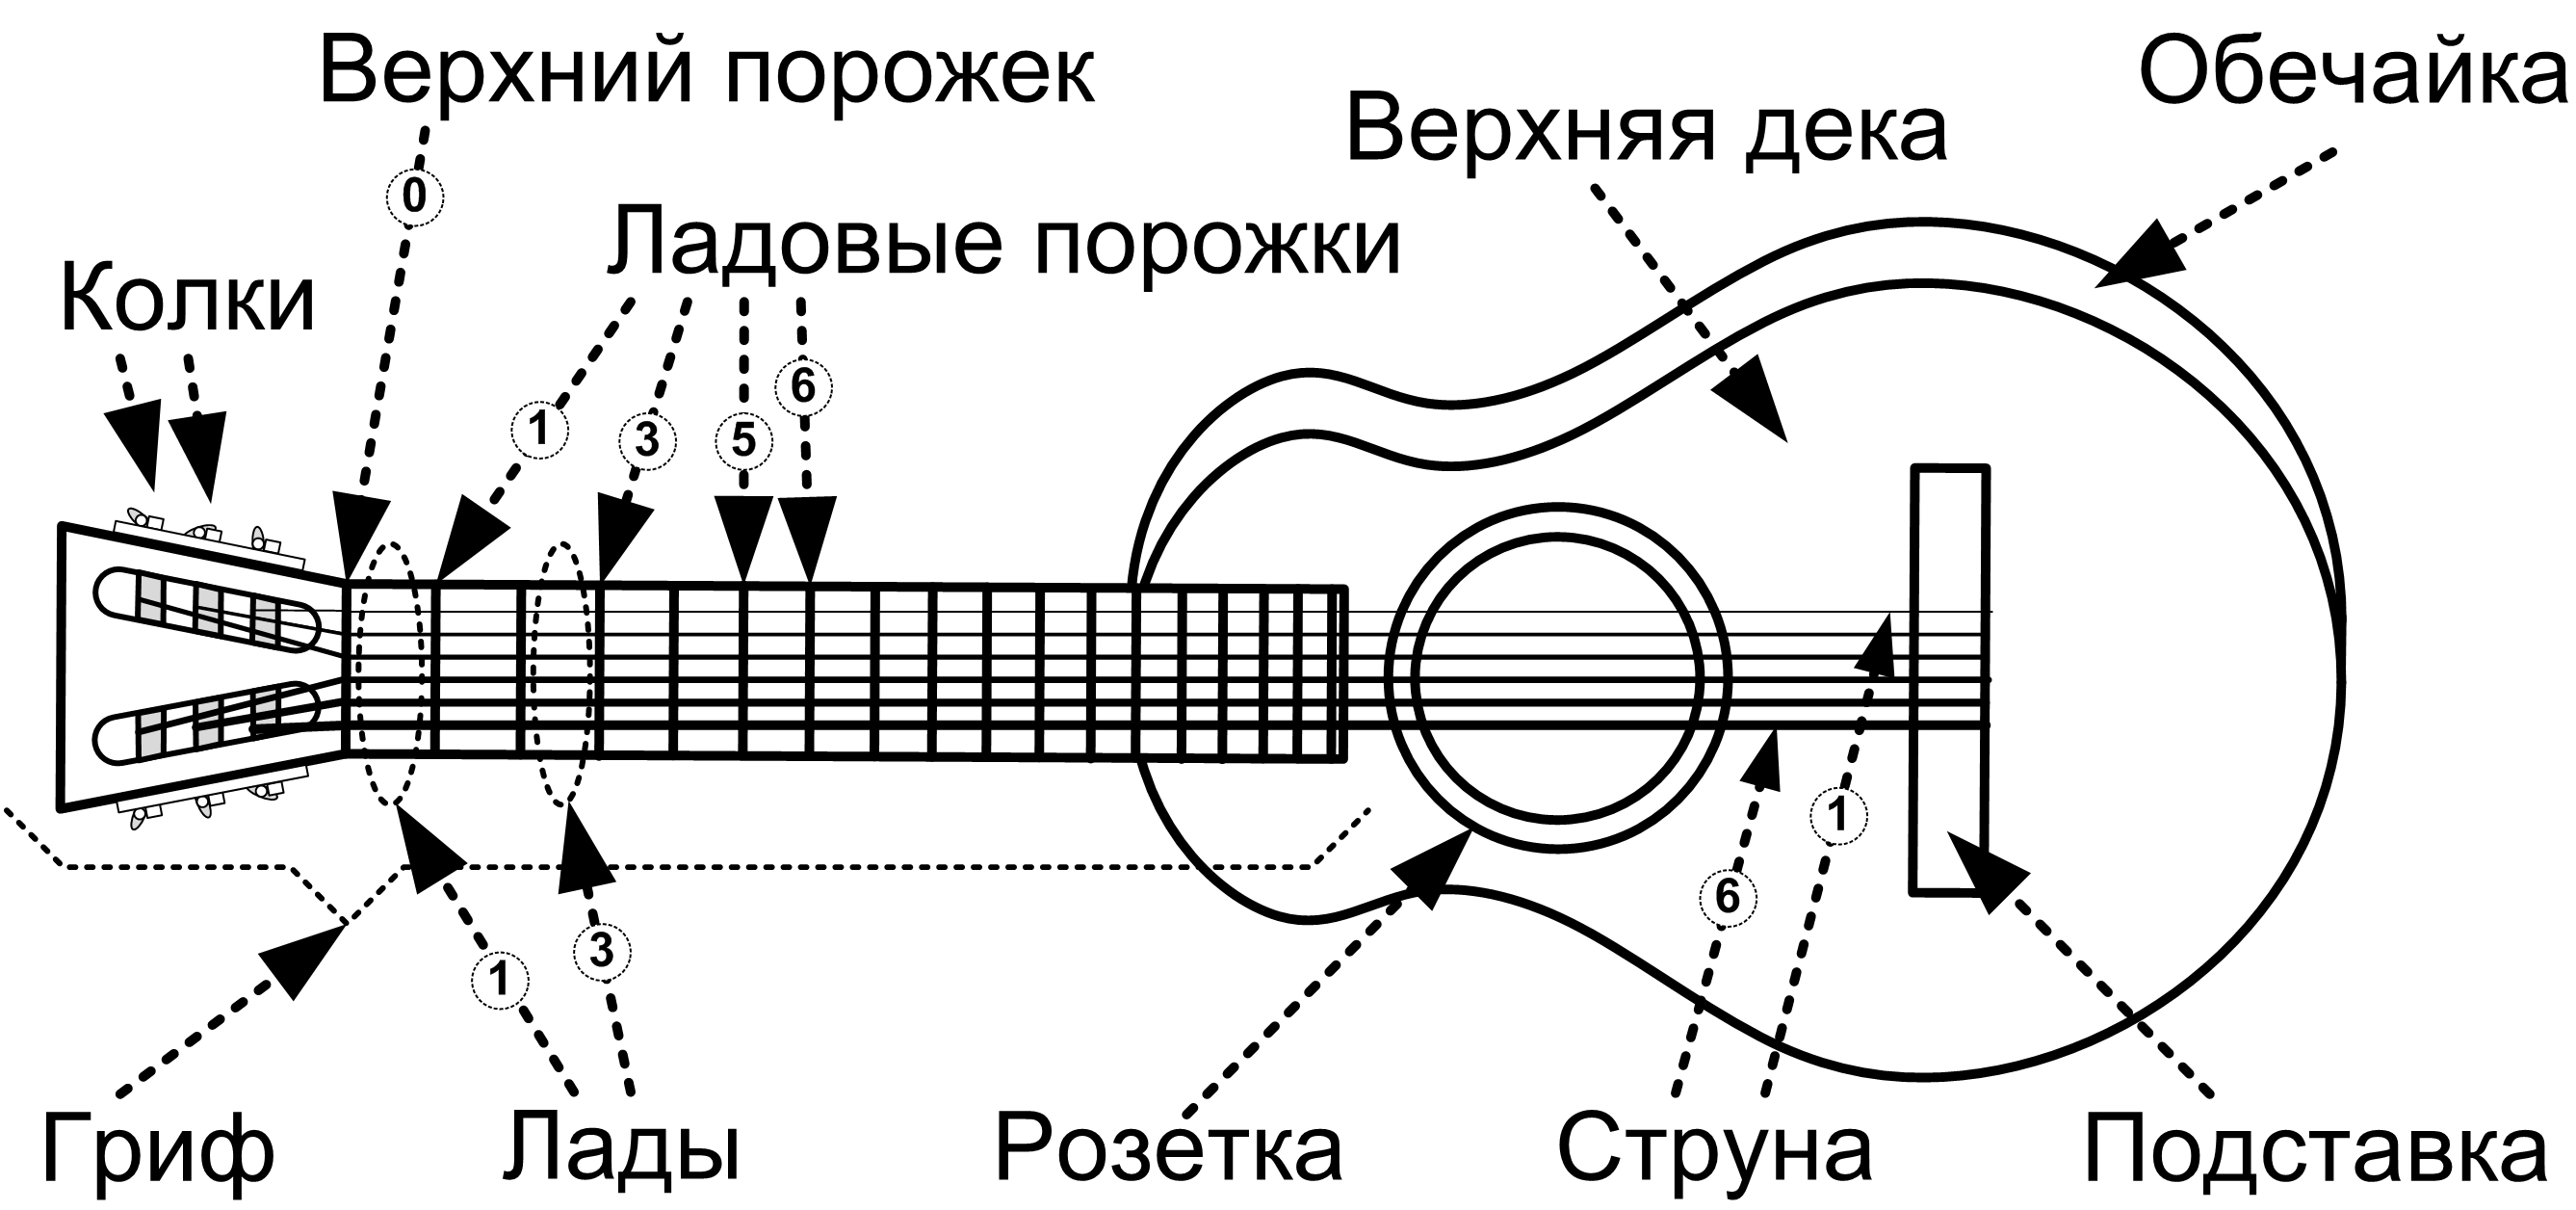
\includegraphics{fig/guitar-construction} 
    \caption{Устройство гитары}\label{fig:guitarConstruction}
\end{figure} 

Любая открытая\footnote{То есть не зажатая ни на каком ладу} струна гитары звучит строго определенной нотой (о настройке гитары поговорим позже). Лады на грифе (промежутки между порожками), равно как и \emph{ладовые порожки} считаются от \emph{верхнего} порожка: 1,2,3,\ldots и т.д. То есть <<зажать струну на первом ладу>> значит, что вы ставите палец на струну, на первый лад, то есть между верхним порожком и первым ладовым\footnote{Чем ближе к первому ладовому, тем лучше. Таким образом и звук будет чище, и рука уставать будет меньше. Ставить палец сверху на порожек не стоит --- звук будет <<глохнуть>>. Правда иногда именно это и требуется. Но в начале обучения стоит ставить палец на ладу ближе к тому порожку, от которого идет <<звучащая>> часть струны. Добивайтесь чистого звука.} и нажимаете до тех пор, пока струна не прижмётся к первому ладовому порожку. Но нам важно сейчас не то, как правильно зажимать струну. 

Важно понять, что каждый следующий лад повышает звук на струне на <<полутон>>. В октаве 12 нот и каждая звучит на струне на своём ладу. На дветадцатом ладу звучит нота открытой струны, только выше на октаву.

Из физики известно, что частота колебаний струны обратно пропорциональна её длине\footnote{Надо честно заметить, что частота колебаний струны зависит также и от силы её натяжения, которая меняется, когда струну <<зажимают>> на ладу. Но это влияние столь незначительно, что им можно пренебречь.}. Стало быть, чтобы частота издаваемого струной звука \emph{увеличилась} вдвое (а языком музыки --- чтобы нота зазвучала октавой выше), надо вдвое \emph{укоротить} струну. 

Зажимая струну на 12 ладу (языком музыки --- повышая ноту открытой струны на октаву), вы укарачиваете звучащую часть струны вдвое. Линейка в помощь, если не верите\footnote{Конечно нужно мерять только звучащую (колеблющуюся часть) струны от опоры на подставке до 12-го ладового порожка.}.

Конечно, частота колебаний струны зависит также и от силы её натяжения. Сила натяжения струны регулируется колками на грифе, когда гитару настраивают. Играя, гитарист только меняет длину звучащего участка струны, зажимая струны на ладах. Редкие психи\footnote{Конечно, имелось в виду: \emph{мастера}! Прим. ред.} крутят колок во время исполнения, добиваясь сомнительных\footnote{Конечно, имелось в виду: \emph{удивительных}! Прим. ред.} эффектов.

Исходя из того, что частота каждой следующей ноты в $\sqrt[12]{2}$ больше предыдущей, запишем формулу длины струны ($L$) от места крепления струны к подставке до $n$-го ладового порожка:

\[L(n)=\frac{L}{(\sqrt[12]{2})^n},\]
где $n$ - номер лада ($0$-й лад соответствует открытой струне), а $L$ --- общая длина струны от подставки до верхнего порожка.


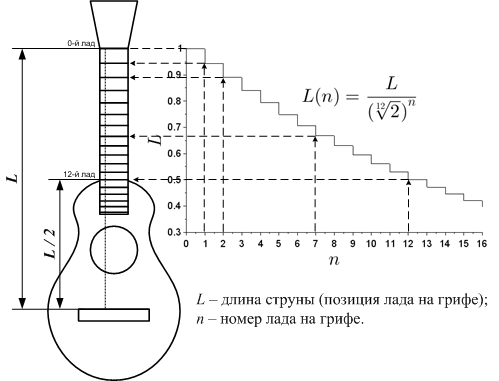
\includegraphics{fig/string-length.png}


Из картинки, надеюсь, ясно, почему ладовые порожки на гитаре расположены не на равном расстоянии друг от друга.

Кстати, некоторые ушастые выпендрёжники говорят, что различают своим сверхмузыкальным слухом больше 12 нот в октаве! И им мало 12 ладов! Есть спрос --- есть предложение: на некоторых гитарах можно заметить дополнительные ладовые порожки между <<каноническими>>, которые позволяют <<всунуть>> дополнительную ноту.


\section{Запись гитарных нот на бумаге}

Чтобы записать ноты, купите нотную тетрадь или на обычном листе начертите нотоносец --- пять параллельных, расположенных друг под другом через равные интервалы (около двух миллиметров) линий:
 

Традиционно ноты для шестиструнной гитаре записываются в скрипичном ключе, который своим хвостиком огибает вторую снизу линию нотоносца, на которой располагется Соль \emph{малой} октавы\footnote{Для других музыкальных инструментов, в первую очередь, для фортепиано, скрипичный ключ показывает положение Соль \emph{первой} октавы, но для гитары, чтобы использовать один нотоносец, ноты пишут на <<фортепианный>> скрипичный нотоносец на октаву выше.}.


\section{Поиск нот на грифе}

\begin{figure}[!ht]
    \centering
    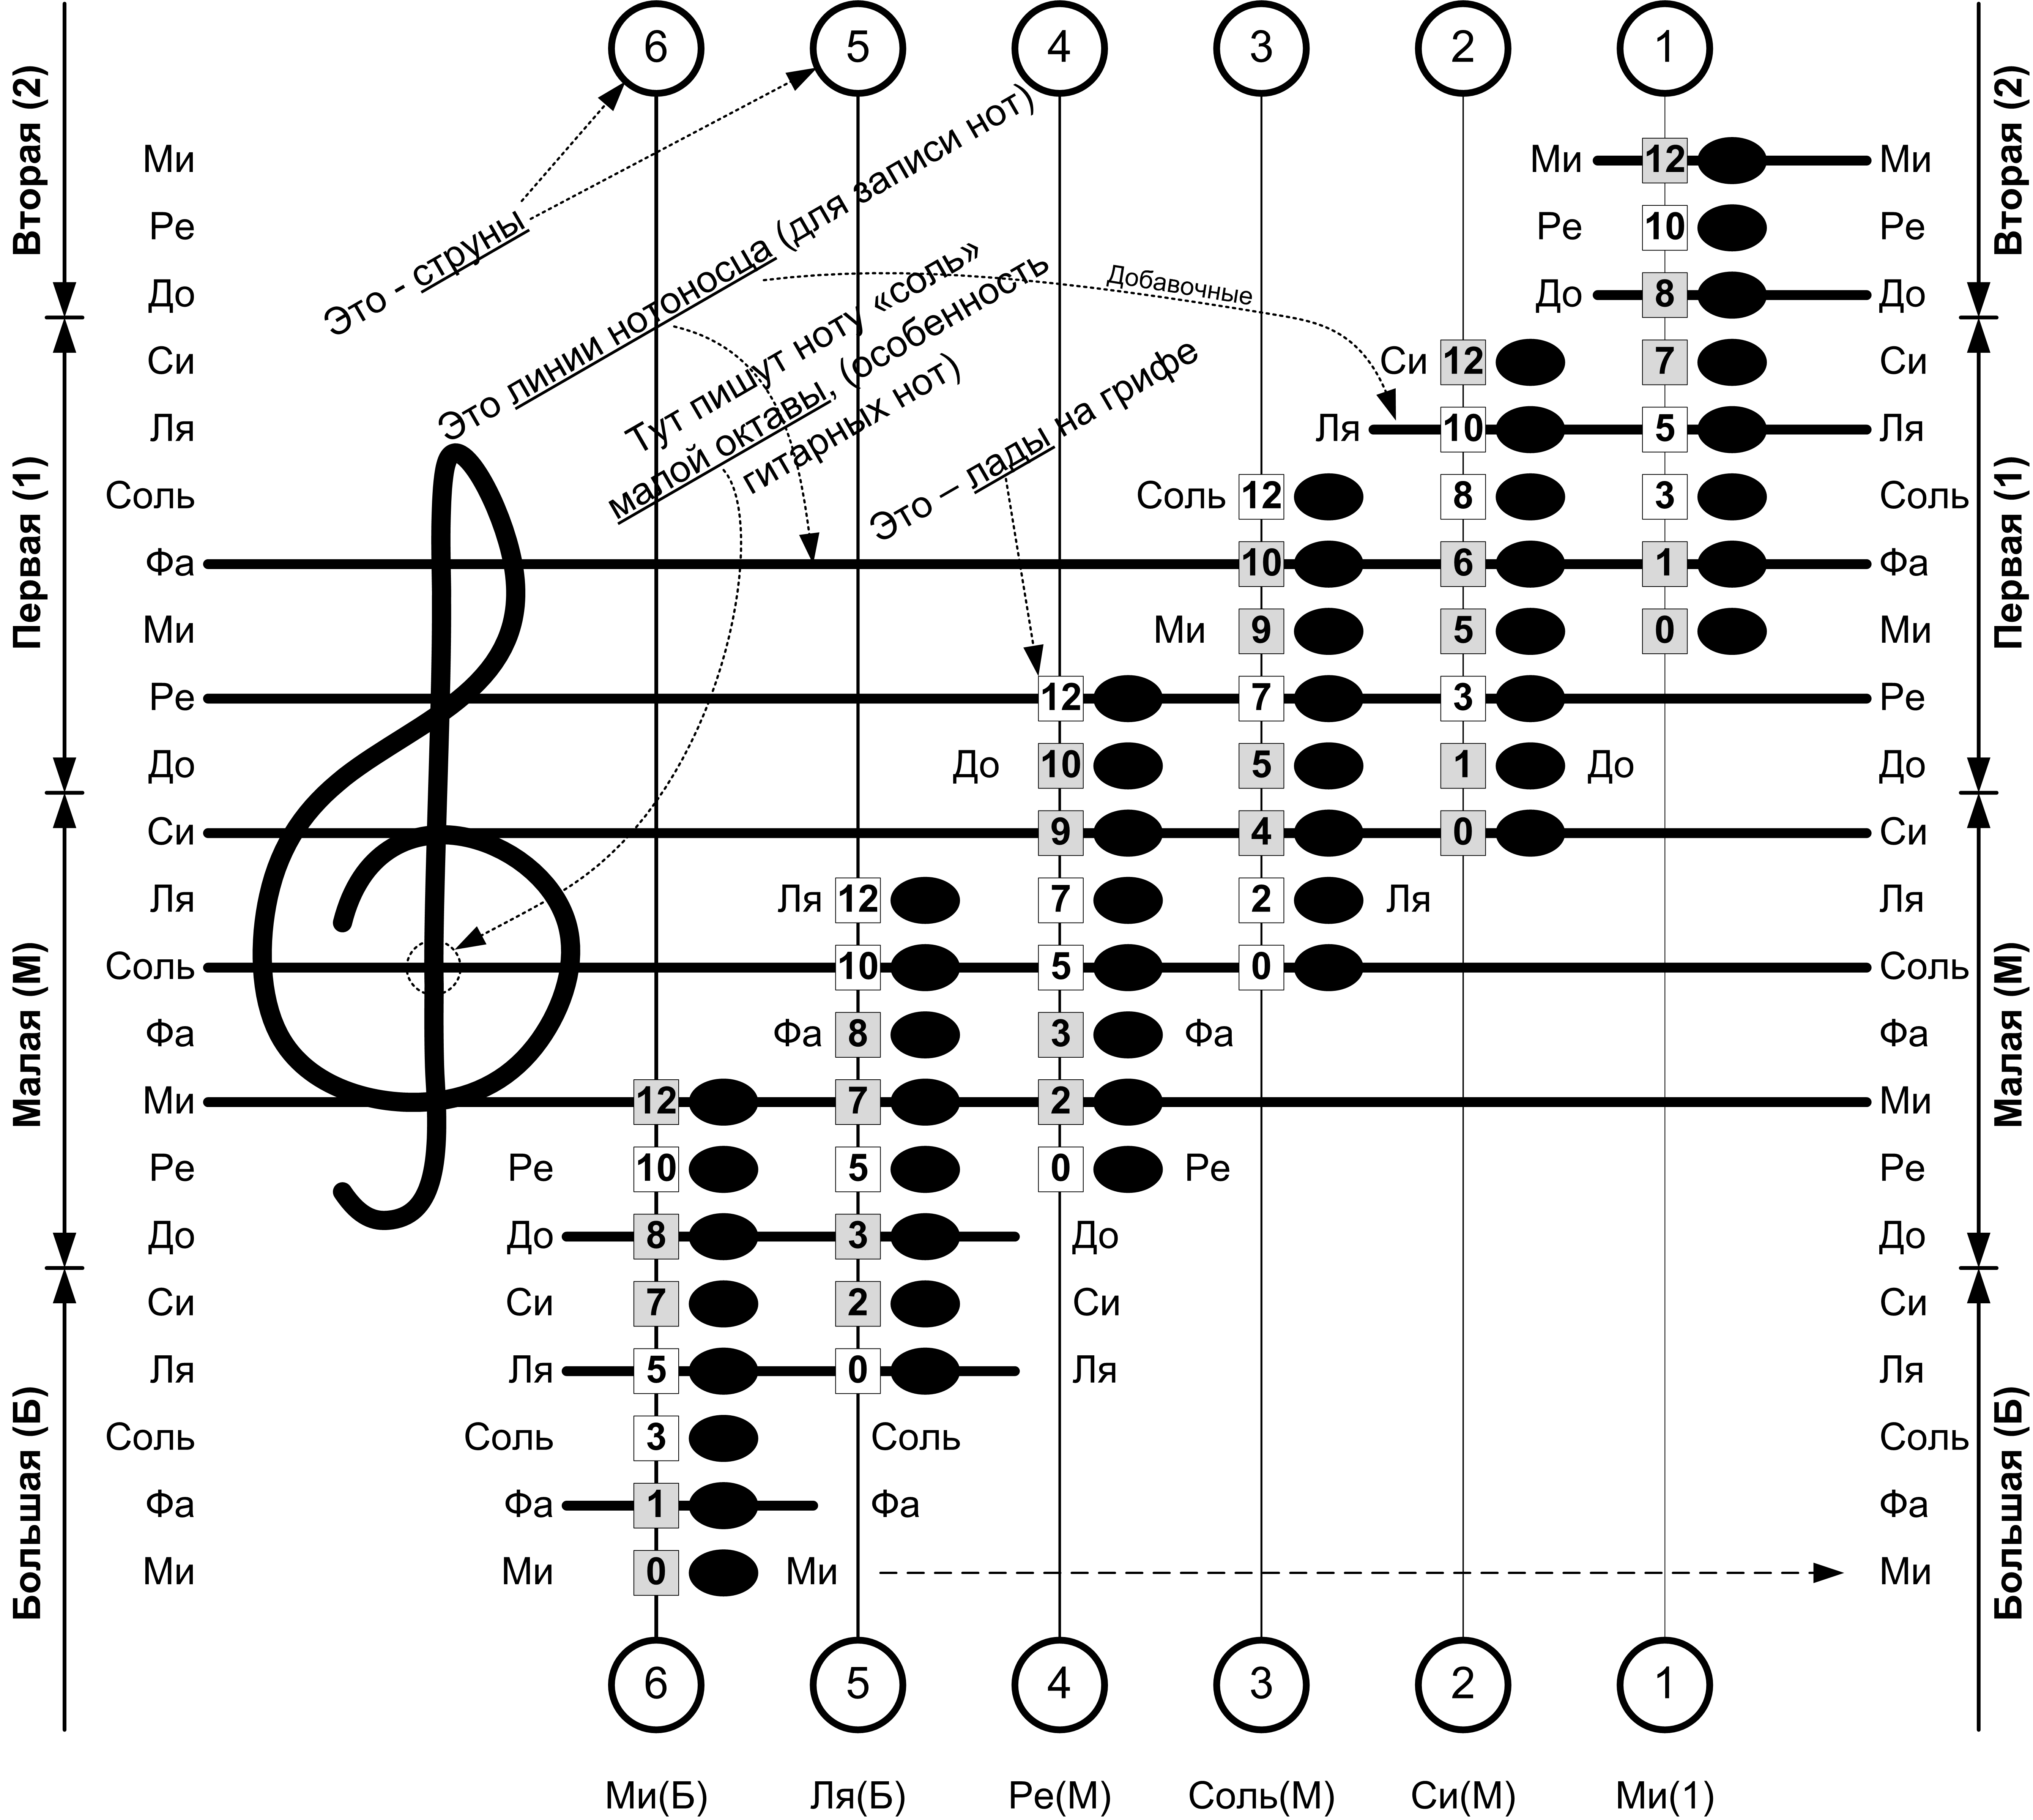
\includegraphics[width=\textwidth]{fig/lad-by-notes} 
    \caption{Ноты на грифе (гриф поперек нотоносца)}\label{fig:ladByNotes}
\end{figure} 

\begin{figure}[!ht]
    \centering
    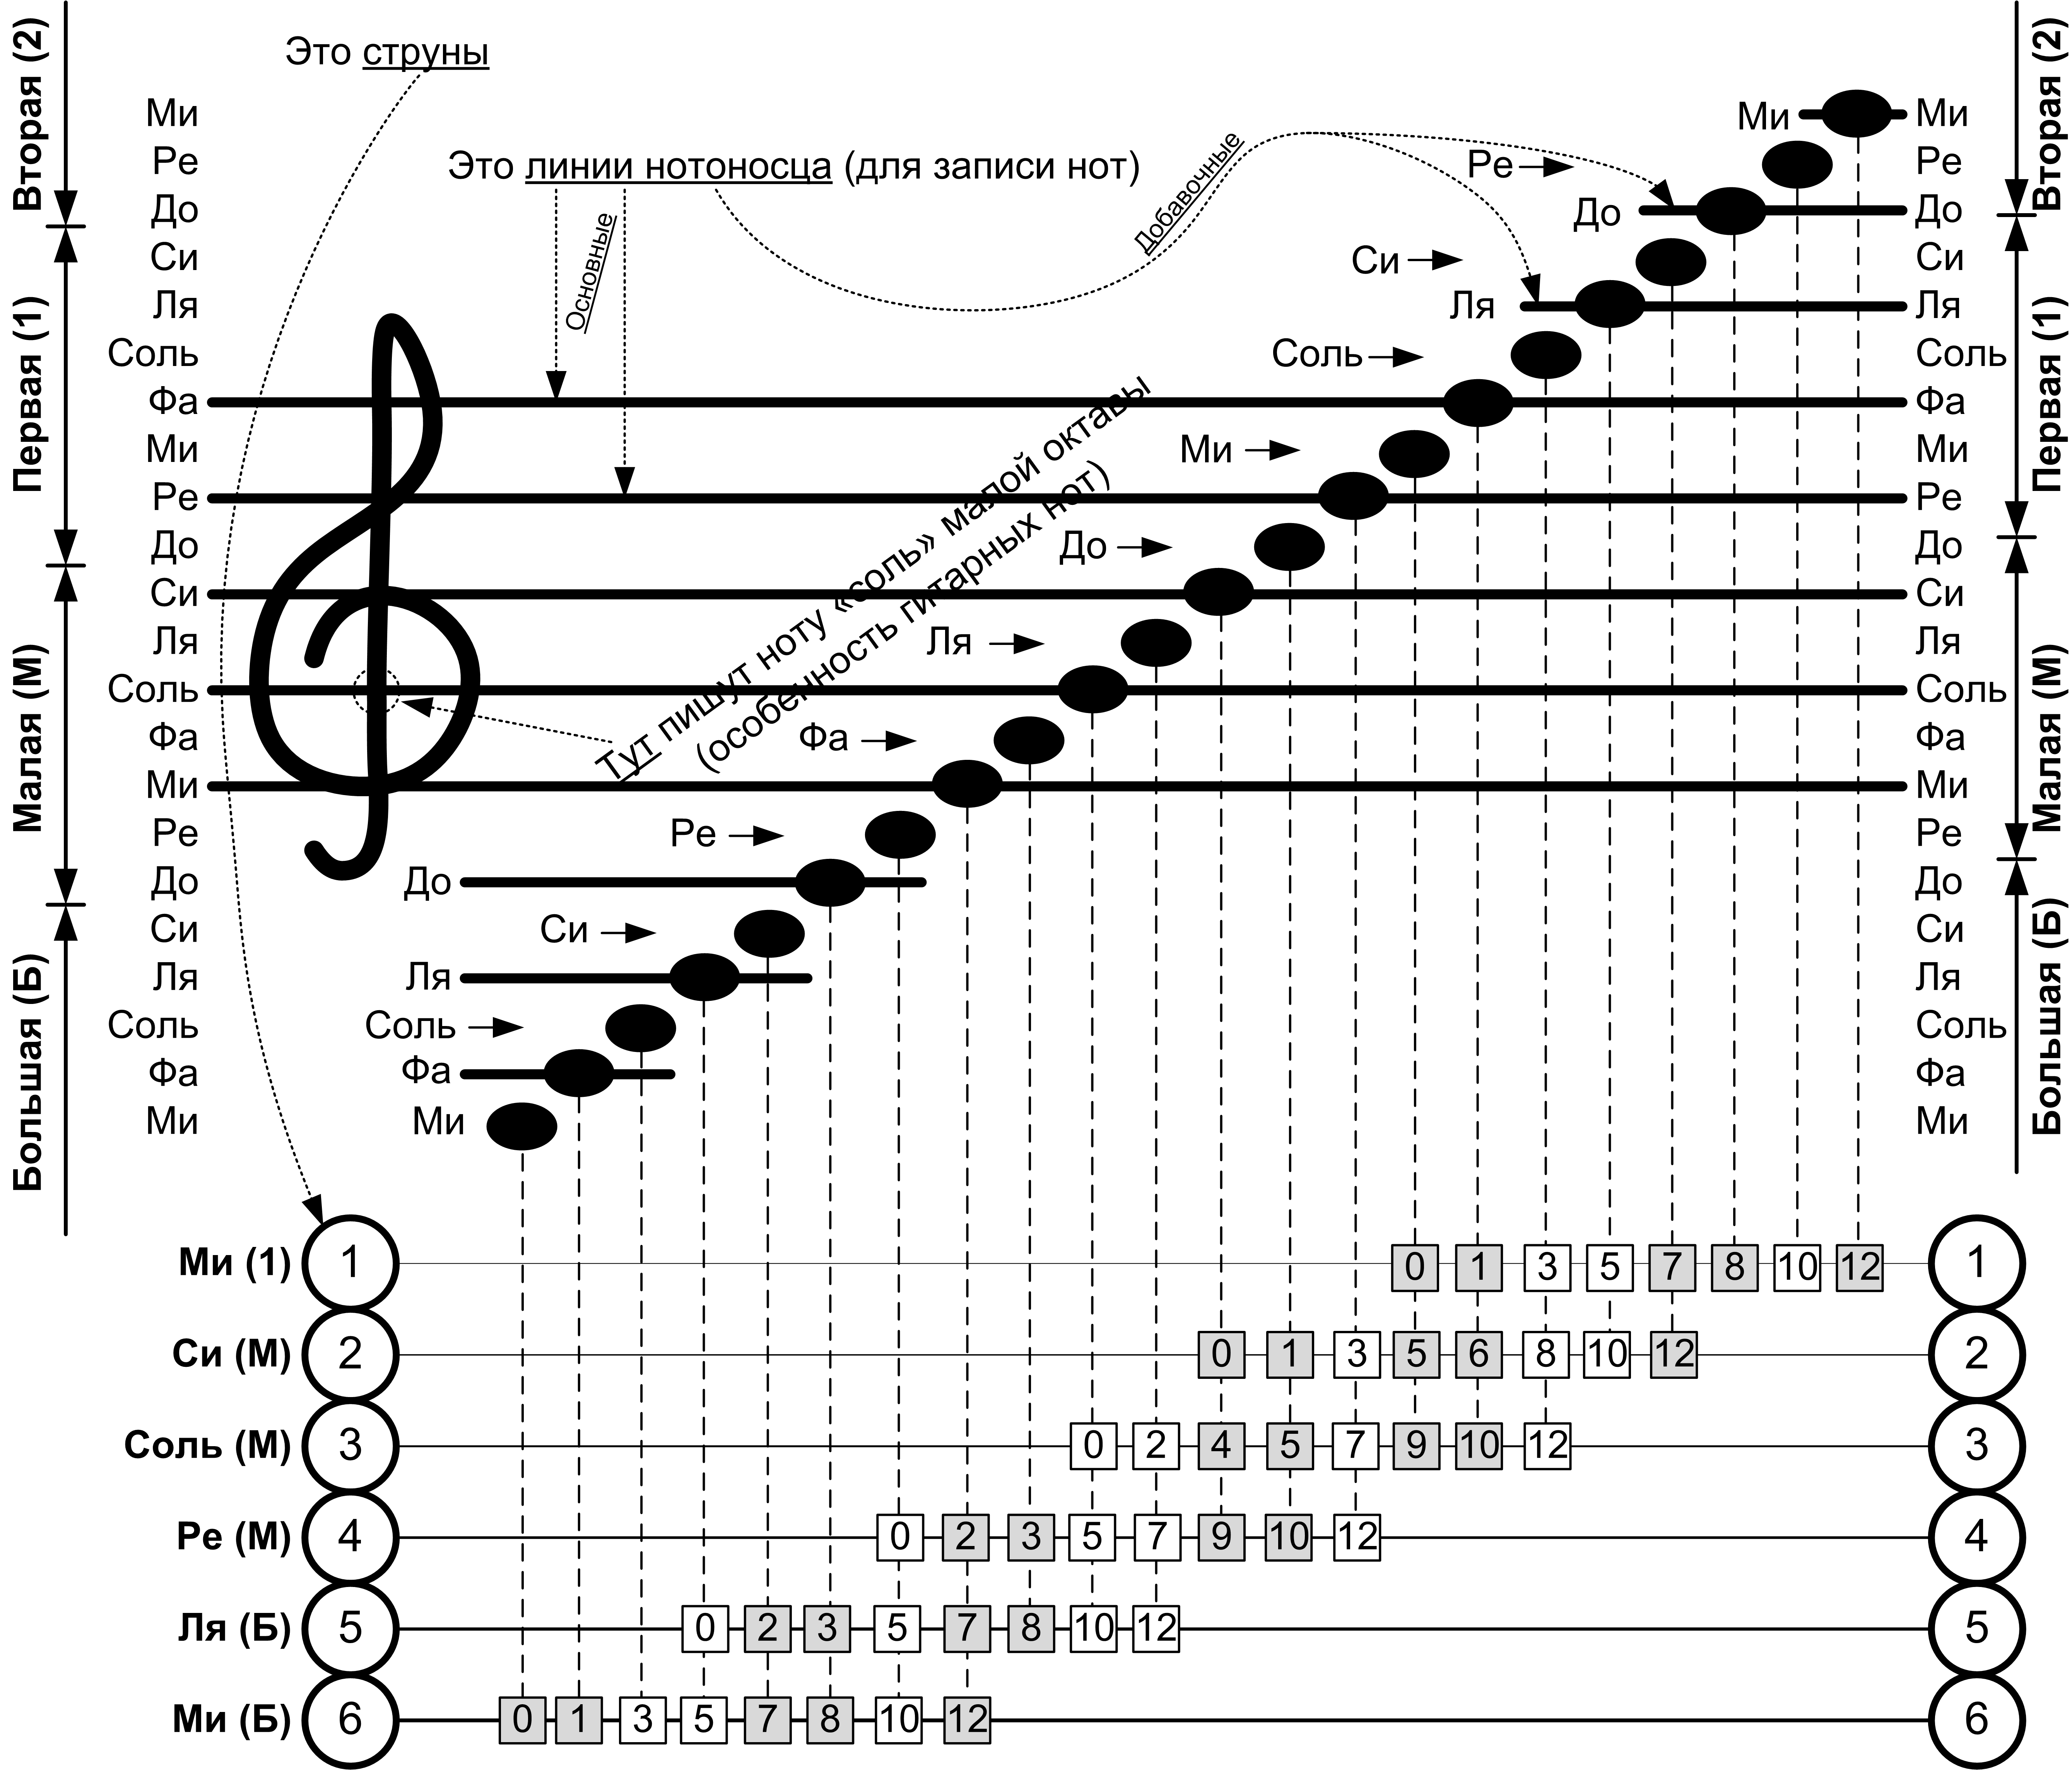
\includegraphics[width=\textwidth]{fig/lad-by-griph} 
    \caption{Ноты на грифе (гриф вдоль нотоносца)}\label{fig:ladByGriph}
\end{figure} 

\begin{figure}[!ht]
    \centering
    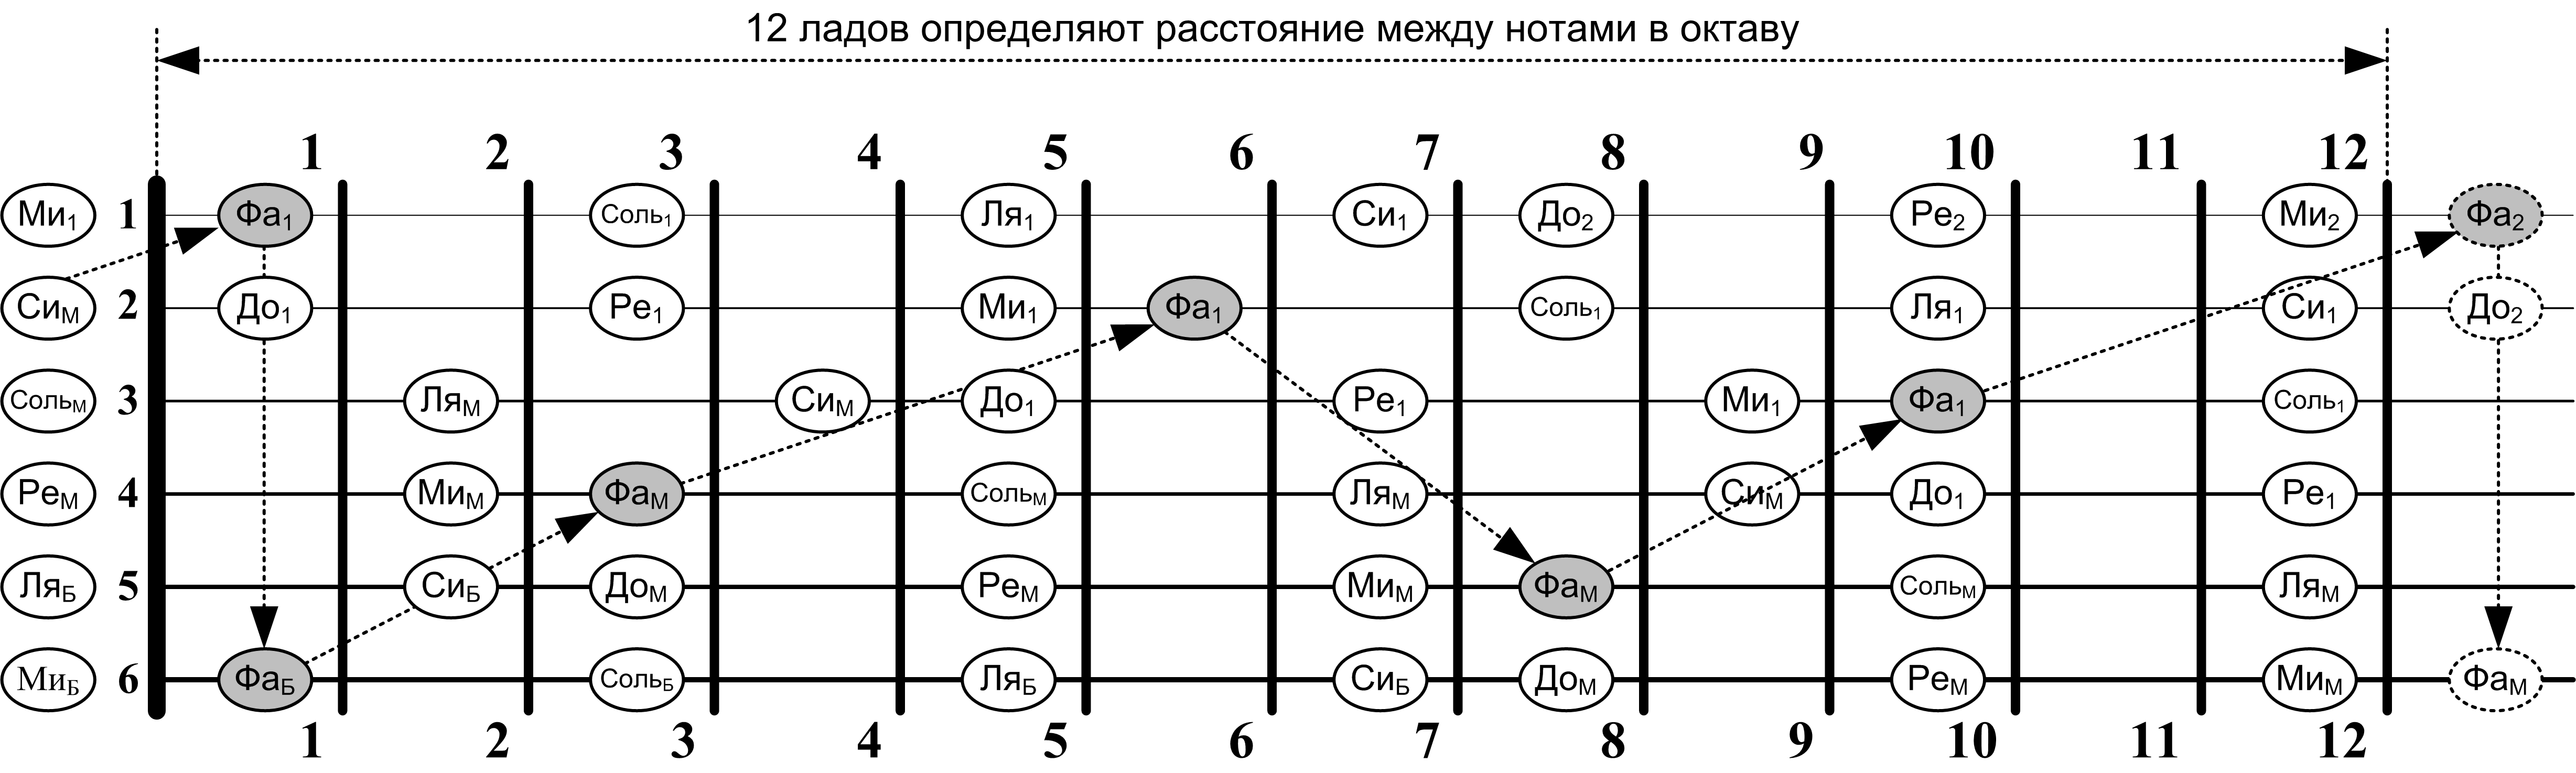
\includegraphics[width=\textwidth]{fig/notes-on-griph} 
    \caption{Ноты на грифе (относительное расположение)}\label{fig:notesOnGriph}
\end{figure} 


\section{Гитарная табулатура}

    %о нотной грамоте пару ласковых
    \chapter*{В заключение}
\addcontentsline{toc}{chapter}{В заключение}

Данный текст подготовлен в издательской системе {\LaTeXe} (автор использовали MiC\TeX.). Эта издательская система является стандартом де факто в научных и технических кругах.

Заинтересовавшимся версткой в {\LaTeX} можно рекомендовать следующие книги: \cite{bib:cotelnikov,bib:baldin}.

Про предшественника {\LaTeX} --- программу {\TeX} следует читать бестселлер от автора\footnote{{\TeX} на самом деле является ядром \LaTeX} \cite{bib:knuth:AllAbout}.
    %заключение
    
    \bibliographystyle{plain}
    \bibliography{./bibliobase}
\end{document} %конец документа
